\documentclass[10pt, a4paper]{article}

\usepackage{ctex}
\usepackage{xeCJK}
\usepackage{caption}
\usepackage{geometry}
\geometry{
    left = 0.6in,
    right = 0.6in,
    top = 0.8in,
    bottom = .6in
}
\usepackage{amssymb}
\usepackage{amsbsy}
\usepackage{amsmath}
\usepackage{xcolor}
\usepackage{mathrsfs}
\usepackage{graphicx}
\usepackage{pifont}
\usepackage{tasks}
\settasks{
    label = \textcolor{purple}{\Alph*.},
    label-width = 14pt
}
\pagestyle{empty}

\newcommand{\Title}[3]{
    \begin{center}
        \Large \textbf{中国电子学会 #1~年~#2~月 Scratch~#3级考试}
    \end{center}
}
\newcommand{\TimeAndName}[1]{
    \begin{center}
        考试时间:~#1~ 分钟 \qquad\qquad\qquad\qquad 姓名:\underline{\quad\quad\quad\quad}
    \end{center}
}
\newcommand{\hq}{\hfill(\qquad)}

\begin{document}
    \Title{2022}{12}{二} % 标题
    \TimeAndName{60} % 考试时间及姓名

    % 单选题
    \vspace{2mm}
    {\noindent\textbf{第一部分、单选题(共 25 题,每题 2 分,共50分.)}}
    \begin{enumerate}
        % 1
        \item 一个骰子,从3个不同角度看过去的点数如图所示,请问5的对面是什么点数? \hq
        \begin{tasks}(4)
            \task 1
            \task 3
            \task 4
            \task 6
        \end{tasks}

        % 2
        \item 明明想做一个大鱼吃小鱼的游戏,下列哪个程序能实现鲨鱼吃到小黄鱼变大10,吃到小红鱼变大20,吃到小蓝鱼变大30?\hq
        \begin{tasks}(4)
            \task 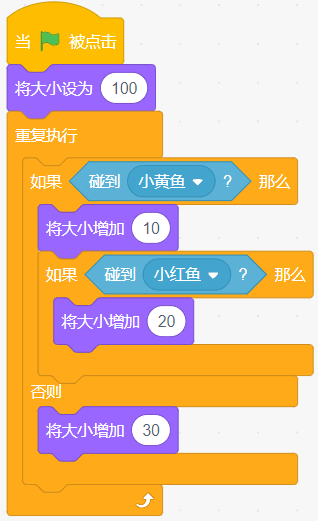
\includegraphics[width=.15\textwidth]{figure/2a.png}
            \task 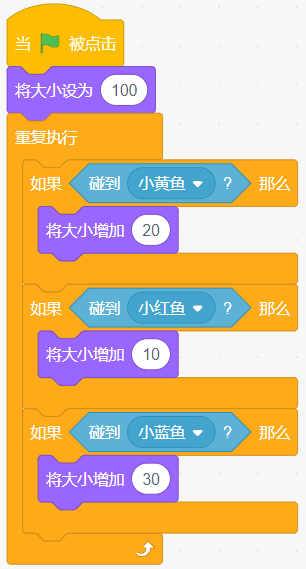
\includegraphics[width=.132\textwidth]{figure/2b.png}
            \task 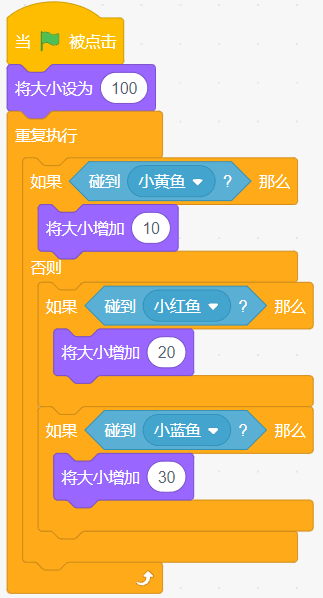
\includegraphics[width=.135\textwidth]{figure/2c.png}
            \task 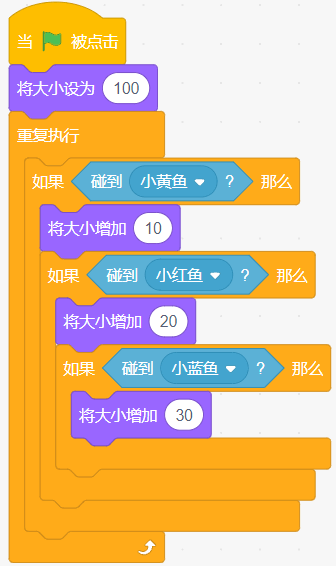
\includegraphics[width=.15\textwidth]{figure/2d.png}
        \end{tasks}

        \begin{figure}[htbp]
            \centering
            \begin{minipage}[t]{.2\textwidth}
                \centering
                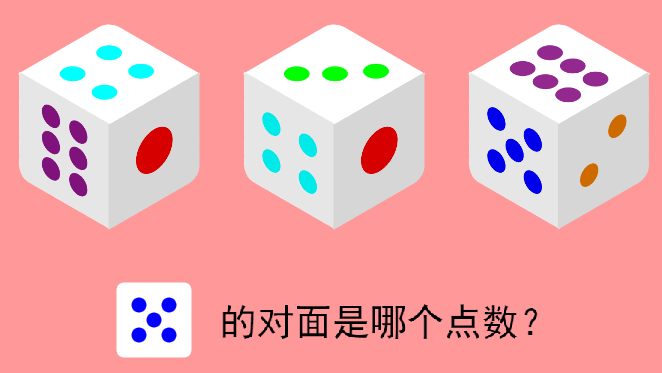
\includegraphics[width=\textwidth]{figure/1.png}
                \caption*{第 1 题}
            \end{minipage}
            \begin{minipage}[t]{.15\textwidth}
                \centering
                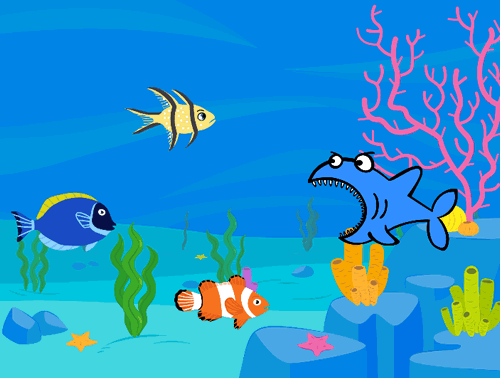
\includegraphics[width=\textwidth]{figure/2.png}
                \caption*{第 2 题}
            \end{minipage}
            \begin{minipage}[t]{.16\textwidth}
                \centering
                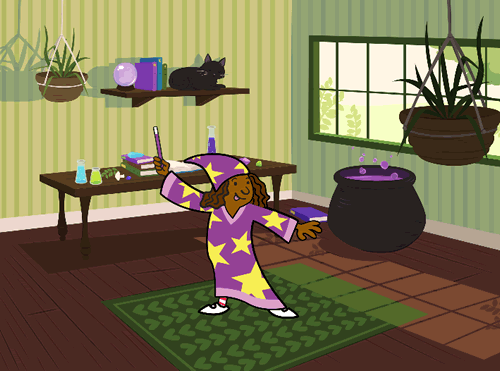
\includegraphics[width=\textwidth]{figure/3.png}
                \caption*{第 3 题}
            \end{minipage}
            \begin{minipage}[t]{.31\textwidth}
                \centering
                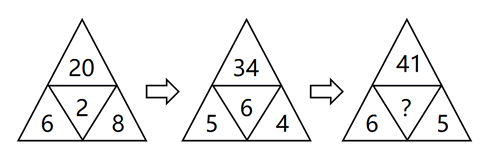
\includegraphics[width=\textwidth]{figure/6.png}
                \caption*{第 6 题}
            \end{minipage}
            \begin{minipage}[t]{.15\textwidth}
                \centering
                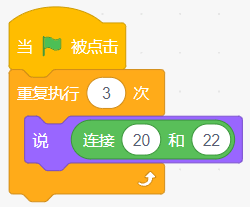
\includegraphics[width=\textwidth]{figure/7.png}
                \caption*{第 7 题}
            \end{minipage}
        \end{figure}

        % 3
        \item 魔法师只有一个造型,下列哪段程序可以实现魔法师念出咒语后,从舞台上消失? \hq
        \begin{tasks}(4)
            \task 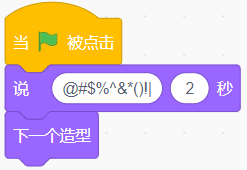
\includegraphics[width=.18\textwidth]{figure/3a.png}
            \task 
\includegraphics[width=.18\textwidth]{figure/3b.png}
            \task 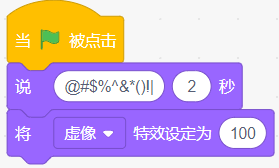
\includegraphics[width=.18\textwidth]{figure/3c.png}
            \task 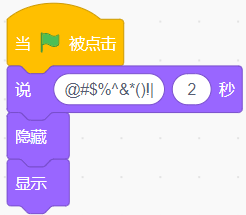
\includegraphics[width=.15\textwidth]{figure/3d.png}
        \end{tasks}

    %     % 4
        \item 有四块水果蛋糕,草莓蛋糕比芒果蛋糕大,草莓蛋糕比菠萝蛋糕小,菠萝蛋糕比火龙果蛋糕小。蛋糕按照从大到小的顺序排列,正确的是?\hq
        \begin{tasks}(2)
            \task 菠萝,草莓,芒果,火龙果
            \task 菠萝,草莓,火龙果,芒果
            \task 火龙果,菠萝,草莓,芒果
            \task 火龙果,菠萝,芒果,草莓
        \end{tasks}

        % 5
        \item 小玉爸爸、小敏爸爸和小霞爸爸三人中有一位教师、一位医生、一位司机,现在只知道,小霞爸爸比司机年龄大,小玉爸爸和医生不同岁,医生比小敏爸爸年龄小。下列说法正确的是? \hq
        \begin{tasks}(4)
            \task 小霞爸爸是教师
            \task 小敏爸爸是教师
            \task 小敏爸爸是司机
            \task 小玉爸爸是医生
        \end{tasks}

        % 6
        \item 观察上图数字规律,“?”处填入的数字应该是?\hq
        \begin{tasks}(4)
            \task 7
            \task 6
            \task 5
            \task 4
        \end{tasks}

        % 7
        \item 运行上图程序,角色说的内容是?\hq
        \begin{tasks}(4)
            \task 202220222022
            \task 2022222
            \task 42
            \task 2022
        \end{tasks}

        \newpage
        % 8
        \item 甲壳虫角色,运行下列程序,说法错误的是?\hq
        \begin{tasks}(2)
            \task 不点击鼠标时,甲壳虫可能会跟随鼠标指针移动
            \task 不点击鼠标时,甲壳虫可能会不停地变化颜色
            \task 不点击鼠标时,甲壳虫移动的同时会变化颜色
            \task 点击鼠标后,甲壳虫不会继续移动
        \end{tasks}

        % 9
        \item 运行下列程序,音量大小调整为?\hq
        \begin{tasks}(4)
            \task 40
            \task 60
            \task 80
            \task 100
        \end{tasks}

        \begin{figure}[htbp]
            \centering
            \begin{minipage}[t]{.18\textwidth}
                \centering
                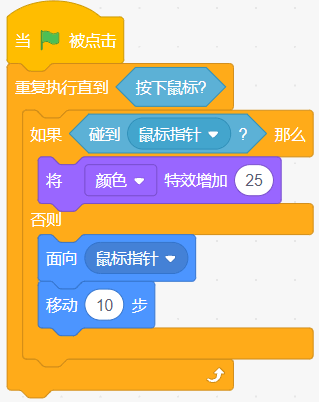
\includegraphics[width=\textwidth]{figure/8.png}
                \caption*{第 8 题}
            \end{minipage}
            \begin{minipage}[t]{.168\textwidth}
                \centering
                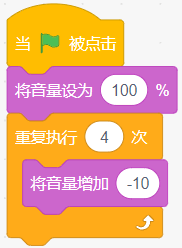
\includegraphics[width=\textwidth]{figure/9.png}
                \caption*{第 9 题}
            \end{minipage}
            \begin{minipage}[t]{.26\textwidth}
                \centering
                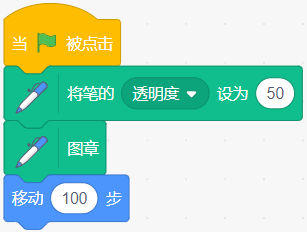
\includegraphics[width=\textwidth]{figure/11.png}
                \caption*{第 11 题}
            \end{minipage}
            \begin{minipage}[t]{.18\textwidth}
                \centering
                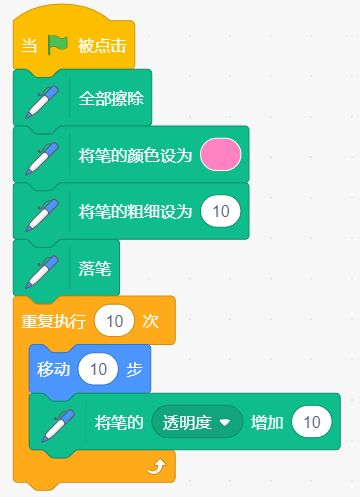
\includegraphics[width=\textwidth]{figure/12.png}
                \caption*{第 12 题}
            \end{minipage}
        \end{figure}

        % 10
        \item 下列哪个程序可以实现小猫角色位置在舞台上不停地变化,按下空格键后停止移动?\hq
        \begin{tasks}(4)
            \task 
\includegraphics[width=.15\textwidth]{figure/10a.png}
            \task 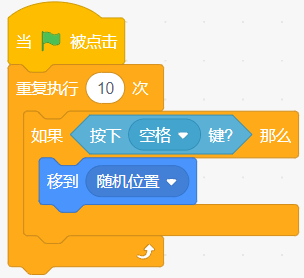
\includegraphics[width=.15\textwidth]{figure/10b.png}
            \task 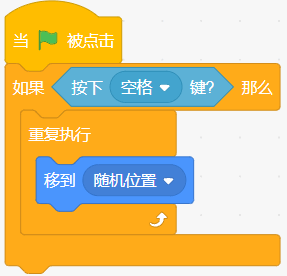
\includegraphics[width=.145\textwidth]{figure/10c.png}
            \task 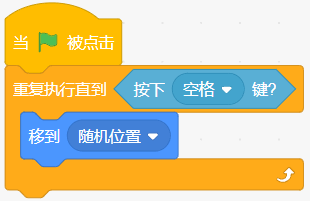
\includegraphics[width=.18\textwidth]{figure/10d.png}
        \end{tasks}

        
        % 11
        \item 运行上图程序,舞台上会显示?\hq
        \begin{tasks}(4)
            \task 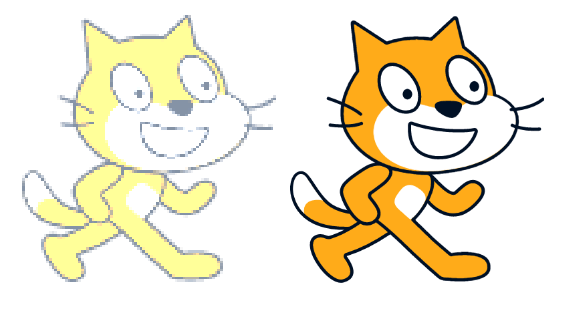
\includegraphics[width=.15\textwidth]{figure/11a.png}
            \task 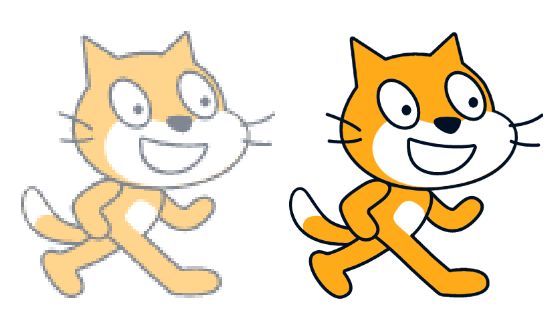
\includegraphics[width=.15\textwidth]{figure/11b.png}
            \task 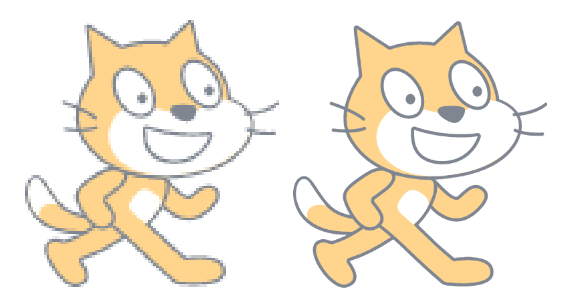
\includegraphics[width=.15\textwidth]{figure/11c.png}
            \task 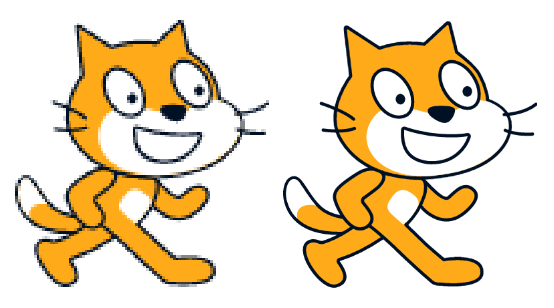
\includegraphics[width=.15\textwidth]{figure/11d.png}
        \end{tasks}

        % 12
        \item 角色初始方向向右,运行上图程序会绘制出什么图形?\hq
        \begin{tasks}(4)
            \task 
\includegraphics[width=.15\textwidth]{figure/12a.png}
            \task 
\includegraphics[width=.15\textwidth]{figure/12b.png}
            \task 
\includegraphics[width=.15\textwidth]{figure/12c.png}
            \task 
\includegraphics[width=.15\textwidth]{figure/12d.png}
        \end{tasks}

        % 13
        \item 小狗和鸡的位置如下图所示,点击绿旗后,小狗会?\hq
        
        \begin{minipage}{.25\textwidth}
            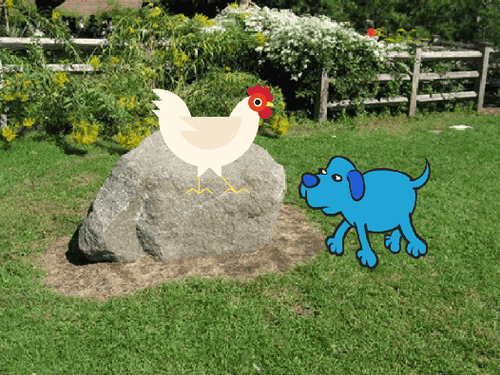
\includegraphics[width=.8\textwidth]{figure/13-1.png}
        \end{minipage}
        \begin{minipage}{.25\textwidth}
            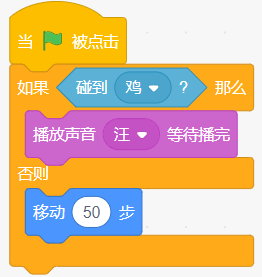
\includegraphics[width=.6\textwidth]{figure/13-2.png}
        \end{minipage}
        \begin{minipage}{.4\textwidth}
            \begin{tasks}
                \task 会“汪”的叫一声
                \task “汪”的叫一声 ,同时移动50步
                \task 没有任何变化
                \task 移动50步
            \end{tasks}
        \end{minipage}
        
        % 14
        \item 舞台有多张背景,棒球运动员程序如下图所示,“颜色碰到”积木中的颜色分别为球棒的颜色和棒球的颜色,点击绿旗后,下列选项正确的是?\hq
        
        \begin{minipage}{.25\textwidth}
            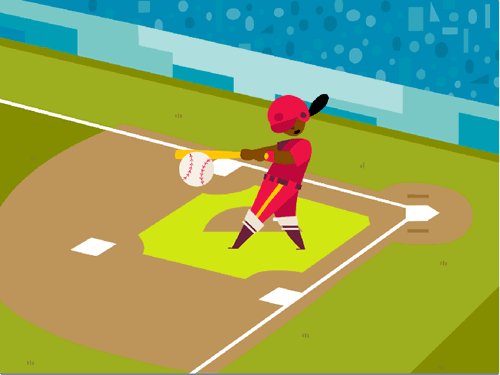
\includegraphics[width=.8\textwidth]{figure/14-1.png}
        \end{minipage}
        \begin{minipage}{.25\textwidth}
            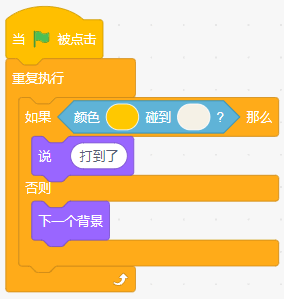
\includegraphics[width=.6\textwidth]{figure/14-2.png}
        \end{minipage}
        \begin{minipage}{.4\textwidth}
            \begin{tasks}
                \task 棒球会一直说“打到了”
                \task 舞台会不停地切换背景
                \task 棒球运动员会一直说“打到了”
                \task 棒球运动员会一直不停地切换造型
            \end{tasks}
        \end{minipage}

        \newpage
        % 15
        \item 小猫和小狗在玩球,位置如下图所示,下列程序不能让小猫在碰到球时,说出“我踢到球了”的是?\hq
        \begin{tasks}(4)
            \task 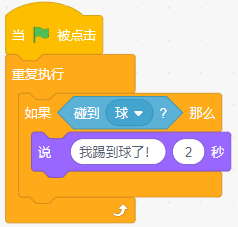
\includegraphics[width=.15\textwidth]{figure/15a.png}
            \task 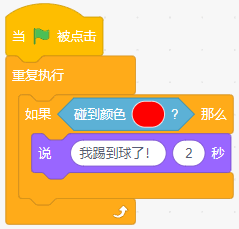
\includegraphics[width=.15\textwidth]{figure/15b.png}
            \task 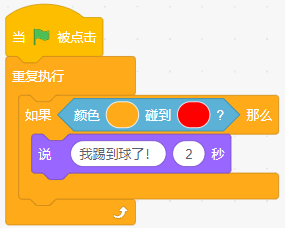
\includegraphics[width=.17\textwidth]{figure/15c.png}
            \task 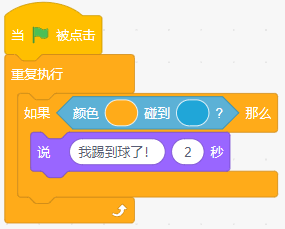
\includegraphics[width=.17\textwidth]{figure/15d.png}
        \end{tasks}

        % 16
        \item 下列哪个选项的结果大于7?\hq
        \begin{tasks}(4)
            \task 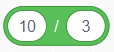
\includegraphics[width=.1\textwidth]{figure/16a.png}
            \task 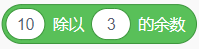
\includegraphics[width=.16\textwidth]{figure/16b.png}
            \task 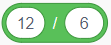
\includegraphics[width=.1\textwidth]{figure/16c.png}
            \task 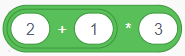
\includegraphics[width=.15\textwidth]{figure/16d.png}
        \end{tasks}

        % 17
        \item 下列哪个选项的结果积木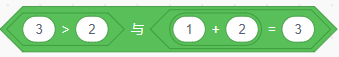
\includegraphics[width=.2\textwidth]{figure/17.png}的结果相等?\hq
        \begin{tasks}(4)
            \task 
\includegraphics[width=.18\textwidth]{figure/17a.png}
            \task 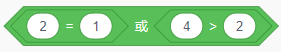
\includegraphics[width=.18\textwidth]{figure/17b.png}
            \task 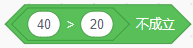
\includegraphics[width=.15\textwidth]{figure/17c.png}
            \task 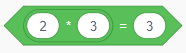
\includegraphics[width=.15\textwidth]{figure/17d.png}
        \end{tasks}

        \begin{figure}[htbp]
            \centering
            \begin{minipage}[t]{.25\textwidth}
                \centering
                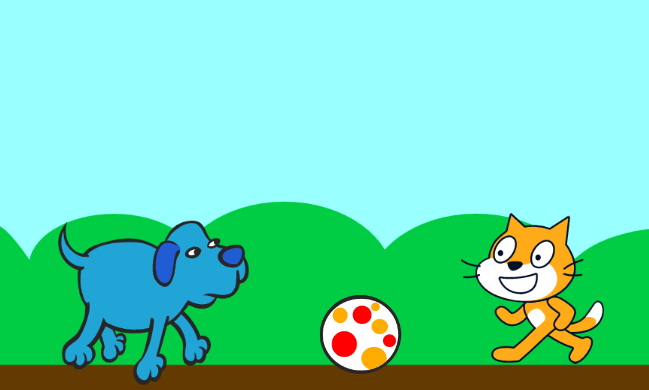
\includegraphics[width=\textwidth]{figure/15.png}
                \caption*{第 15 题}
            \end{minipage}
            \begin{minipage}[t]{.255\textwidth}
                \centering
                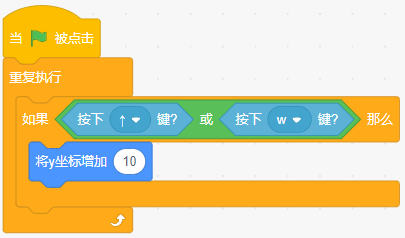
\includegraphics[width=\textwidth]{figure/18.png}
                \caption*{第 18 题}
            \end{minipage}
            \begin{minipage}[t]{.2\textwidth}
                \centering
                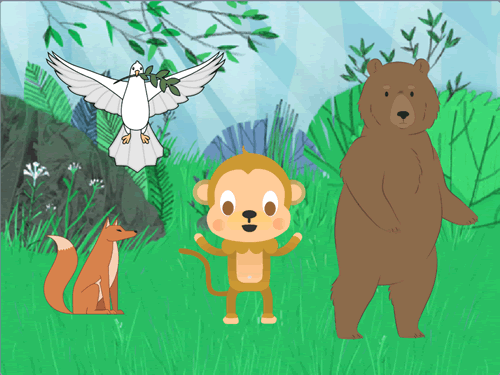
\includegraphics[width=\textwidth]{figure/19.png}
                \caption*{第 19 题}
            \end{minipage}
            \begin{minipage}[t]{.15\textwidth}
                \centering
                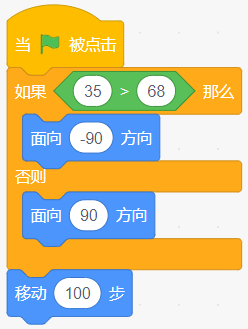
\includegraphics[width=\textwidth]{figure/21.png}
                \caption*{第 21 题}
            \end{minipage}
        \end{figure}

        % 18
        \item 小猫角色运行下列程序,说法正确的是?\hq
        \begin{tasks}(2)
            \task 只按下w键,小猫就能向下走
            \task 要同时按下↑键和w键,小猫才能向上走
            \task 只按下↑键,小猫就能向上走
            \task 不按任何键,小猫就能向上走
        \end{tasks}

        % 19
        \item 动物王国要举办音乐会,下列哪个程序能实现音乐连续不停地播放,并且每播放一次声音都逐渐减弱?\hq
        \begin{tasks}(4)
            \task \includegraphics[width=.12\textwidth]{figure/19a.png}
            \task \includegraphics[width=.16\textwidth]{figure/19b.png}
            \task \includegraphics[width=.16\textwidth]{figure/19c.png}
            \task \includegraphics[width=.16\textwidth]{figure/19d.png}
        \end{tasks}

        % 20
        \item 架子鼓和电子琴的程序如下图,哪个选项可以让架子鼓和电子琴同时停止声音播放,不再听到任何声音?\hq
        
        \begin{minipage}{.2\textwidth}
            \centering
            \includegraphics[width=\textwidth]{figure/20-1.png}
        \end{minipage}
        \begin{minipage}{.2\textwidth}
            \centering
            \includegraphics[width=\textwidth]{figure/20-2.png}
        \end{minipage}
        \begin{minipage}{.48\textwidth}
            \begin{tasks}(2)
                \task \includegraphics[width=.15\textwidth]{figure/20a.png}
                \task \includegraphics[width=.25\textwidth]{figure/20b.png}
                \task \includegraphics[width=.25\textwidth]{figure/20c.png}
                \task \includegraphics[width=.2\textwidth]{figure/20d.png}
            \end{tasks}
        \end{minipage}

        % 21
        \item 小猫初始位置在舞台中心,面向右,运行下列程序,舞台上会显示?\hq
        \begin{tasks}(4)
            \task \includegraphics[width=.18\textwidth]{figure/21a.png}
            \task \includegraphics[width=.18\textwidth]{figure/21b.png}
            \task \includegraphics[width=.18\textwidth]{figure/21c.png}
            \task \includegraphics[width=.18\textwidth]{figure/21d.png}
        \end{tasks}

        \newpage
        % 22
        \item 在“密室寻宝”游戏中,下列哪个积木可以实现将钥匙藏在短袖下? \hq
        
        \begin{minipage}{.21\textwidth}
            \centering
            \includegraphics[width=.7\textwidth]{figure/22.png}
        \end{minipage}
        \begin{minipage}{.7\textwidth}
            \begin{tasks}(2)
                \task \includegraphics[width=.14\textwidth]{figure/22a.png}
                \task \includegraphics[width=.18\textwidth]{figure/22b.png}
                \task \includegraphics[width=.14\textwidth]{figure/22c.png}
                \task \includegraphics[width=.18\textwidth]{figure/22d.png}
            \end{tasks}
        \end{minipage}

        % 23
        \item 如图所示,苹果成熟后会从树上落下来,苹果落到刺猬身上后,会换成切开造型并停止掉落,下列哪个程序不能实现?\hq
        \begin{tasks}(4)
            \task \includegraphics[width=.15\textwidth]{figure/23a.png}
            \task \includegraphics[width=.18\textwidth]{figure/23b.png}
            \task \includegraphics[width=.165\textwidth]{figure/23c.png}
            \task \includegraphics[width=.18\textwidth]{figure/23d.png}
        \end{tasks}

        \begin{figure}[htbp]
            \centering
            \begin{minipage}[t]{.22\textwidth}
                \centering
                \includegraphics[width=\textwidth]{figure/23.png}
                \caption*{第 23 题}
            \end{minipage}
            \begin{minipage}[t]{.22\textwidth}
                \includegraphics[width=\textwidth]{figure/25.png}
                \caption*{第 25 题}
            \end{minipage}
            \begin{minipage}[t]{.26\textwidth}
                \includegraphics[width=\textwidth]{figure/26.png}
                \caption*{第 26 题}
            \end{minipage}
            \begin{minipage}[t]{.13\textwidth}
                \centering
                \includegraphics[width=\textwidth]{figure/28.png}
                \caption*{第 28 题}
            \end{minipage}
        \end{figure}

        % 24
        \item 妈妈想让小明帮忙买水果,如果有苹果就买苹果,没有苹果就买香蕉,使用下列哪个积木最容易实现?\hq
        \begin{tasks}(4)
            \task \includegraphics[width=.18\textwidth]{figure/24a.png}
            \task \includegraphics[width=.18\textwidth]{figure/24b.png}
            \task \includegraphics[width=.115\textwidth]{figure/24c.png}
            \task \includegraphics[width=.18\textwidth]{figure/24d.png}
        \end{tasks}

        % 25
        \item 小猫想和棕熊打招呼,初始位置如上图所示,两个角色之间的直线距离为300,下列程序不能让小猫走到棕熊面前的是?\hq
        \begin{tasks}(4)
            \task \includegraphics[width=.1\textwidth]{figure/25a.png}
            \task \includegraphics[width=.18\textwidth]{figure/25b.png}
            \task \includegraphics[width=.1\textwidth]{figure/25c.png}
            \task \includegraphics[width=.18\textwidth]{figure/25d.png}
        \end{tasks}
    \end{enumerate}

    % 判断题
    {\noindent\textbf{第二部分、判断题(共 10 题,每题 2 分,共20分.)}}
    \begin{enumerate}
        \setcounter{enumi}{25}
        % 26
        \item 上图两段程序实现的效果是一样的。\hq

        % 27
        \item 14个同学依次报数,报单数的按从小到大站一排,报双数的按从小到大站一排。那么单数排的第3个同学是5号,双数排的第5个同学是10号。\hq

        % 28
        \item 青蛙是森林中的跳跃高手,程序如上图所示,那么点击绿旗之后,青蛙会一直上下跳跃,直到按下鼠标,它才会停止。\hq

        \newpage
        % 29
        \item 男孩和足球的初始位置如图所示,已知每个格子的边长为30,运行下列这段程序,男孩可以碰到球。\hq

        \begin{figure}[htbp]
            \centering
            \begin{minipage}[t]{.4\textwidth}
                \centering
                \begin{minipage}[t]{.65\textwidth}
                    \centering
                    \includegraphics[width=\textwidth]{figure/29-1.png}
                \end{minipage}
                \begin{minipage}[t]{.25\textwidth}
                    \centering
                    \includegraphics[width=\textwidth]{figure/29-2.png}
                \end{minipage}
                \caption*{第 29 题}
            \end{minipage}
            \begin{minipage}[t]{.13\textwidth}
                \centering
                \includegraphics[width=\textwidth]{figure/30.png}
                \caption*{第 30 题}
            \end{minipage}
            \begin{minipage}[t]{.25\textwidth}
                \centering
                \includegraphics[width=\textwidth]{figure/31.png}
                \caption*{第 31 题}
            \end{minipage}
        \end{figure}

        % 30
        \item 运行上图所示程序,可以绘制出一个红色的正方形。\hq

        % 31
        \item 使用上图所示积木可以判断出是否按下了鼠标。\hq

        % 32
        \item 如图积木 \includegraphics[width=.25\textwidth]{figure/32.png} 的运行结果为true。\hq

        % 33
        \item 点击下图中的“响一点”按钮可以使声音变得大一些。\hq
        
        \begin{figure}[htbp]
            \centering
            \begin{minipage}[t]{.3\textwidth}
                \centering
                \includegraphics[width=\textwidth]{figure/33.png}
                \caption*{第 31 题}
            \end{minipage}
            \begin{minipage}[t]{.4\textwidth}
                \centering
                \begin{minipage}[t]{.4\textwidth}
                    \centering
                    \includegraphics[width=\textwidth]{figure/34-1.png}
                \end{minipage}
                \begin{minipage}[t]{.4\textwidth}
                    \centering
                    \includegraphics[width=\textwidth]{figure/34-2.png}
                \end{minipage}
                \caption*{第 34 题}
            \end{minipage}
            \begin{minipage}[t]{.2\textwidth}
                \centering
                \includegraphics[width=\textwidth]{figure/35.png}
                \caption*{第 35 题}
            \end{minipage}
        \end{figure}

        % 34
        \item 水母和小丑鱼的位置如上左图所示,两个角色中都有上右图程序,把鼠标移到角色重叠处按下空格键后,只有小丑鱼会向右移动100步。\hq

        % 35
        \item 运行上图程序,角色说“不对”。\hq
    \end{enumerate}

    \newpage
    {\noindent \textbf{第三部分、编程题(共 2 题,共30分.)}}
    \begin{enumerate}
        \setcounter{enumi}{35}
        
        % 36
        \item 老鹰捉小鸡:
        
        1. 准备工作
        \begin{tasks}[label = (\arabic*)]
            \task 删除默认白色背景,添加背景Farm;
            \task 删除默认角色小猫,添加角色Chick、Griffin。
        \end{tasks}
        2. 功能实现
        \begin{tasks}[label = (\arabic*)]
            \task 角色的初始位置和方向如下图所示;
            \task 老鹰不断向右下移动,碰到边缘就反弹,不能倒立;
            \task 用上、下、左、右键,控制小鸡朝上下左右四个不同的方向移动,不能倒立;
            \task 老鹰碰到小鸡后,老鹰会说“我抓住你了!” 2秒,停止全部脚本;
            \task 小鸡走进鸡舍后,会说“我安全啦!”2秒,然后消失,停止全部脚本。
        \end{tasks}
        \begin{figure}[htbp]
            \centering
            \begin{minipage}[t]{.3\textwidth}
                \centering
                \includegraphics[width=\textwidth]{figure/36-1.png}
            \end{minipage}
            \begin{minipage}[t]{.29\textwidth}
                \centering
                \includegraphics[width=\textwidth]{figure/36-2.png}
            \end{minipage}
            \begin{minipage}[t]{.29\textwidth}
                \centering
                \includegraphics[width=\textwidth]{figure/36-3.png}
            \end{minipage}
        \end{figure}

        %37
        \item 绘制风车:
        
        1. 准备工作
        \begin{tasks}[label = (\arabic*)]
            \task 隐藏默认的小猫角色;
            \task 选择背景:“Xy-grid”。
        \end{tasks}
        2. 功能实现
        \begin{tasks}[label = (\arabic*)]
            \task 小猫角色的初始位置为$(x:0,y:0)$;
            \task 线条粗细为5,三角形的边长为100;
            \task 绘制如下图所示的图形,三角形的颜色分别为绿色、红色、橙色,方向和所示图相同。
        \end{tasks}

        \begin{figure}[htbp]
            \centering
            \includegraphics[width=.4\textwidth]{figure/37.png}
        \end{figure}
    \end{enumerate}
\end{document}